\chapter{Dataset}\label{chapter:Dataset}

\section{Construction}
The main goal is to gather a diverse and high-quality dataset which represents static
real-world HTML/CSS webpages. This includes different layouts, components and contents. 
In the past, there have been different attempts to collect a dataset fullfilling
exactly those requirements.\newline
Two promising examples in this field are \textit{Design2Code} and \textit{Webcode2m}. 
Both have used existing, large datasets and applied different processing steps to 
filter bad examples and remove noise or redundancy from the code. Based on their
dataset curation, both serve as a good base for this thesis.\newline
Therefore, we decided to use both datasets and manually select 53 high-quality data 
entries. Those 53 data entries consist of 28 entries from Design2Code and 25 entries
from Webcode2m. In order to compare them on a fair basis, we only collect webpages 
that have english as their primary language.

\subsection{Content Distribution}
By using data entries of various domains and different layouts, we make sure to get 
a fair representation of the distribution of webpages in the real world. Based on 
our manual selection, we present the domain distribution in a pie chart in Figure 1.

\begin{figure*}[p]
  \centering
  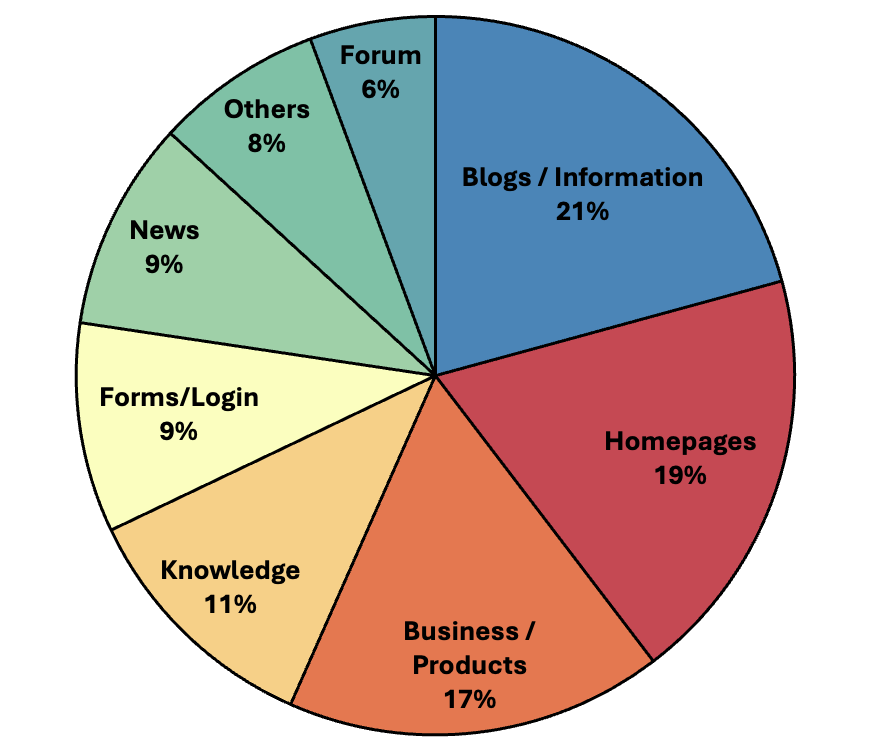
\includegraphics[width=\textwidth]{figures/dataset_distribution.png}
  \caption{Distribution of Topics in Dataset}
  \label{fig:dataset_distribution}
\end{figure*}

\section{Data Mutation}
Due to the fact that Design2Code and Webcode2m use different strategies to purify
their data, it is necessary to align both datasets in order to get a fair comparison.
This includes removing all external dependencies such as multimedia files (e.g. images
, audio, videos, {\ldots}) from the datasets. Furhtermore, this means adding 
placeholders like src=\"placeholder.jpg\" for images or href=\"\#\" for <a> Tags.
Lastly, we remove all of the non-visible content (advertisement-related, hidden) 
of the webpages, because it is not necessary in an Image-to-Code environment and 
could only add negatively to the accessibility score.\newline
In a last step

